\documentclass{article}
\usepackage{amsfonts}
\usepackage{tikz}
\usetikzlibrary{positioning}
\usetikzlibrary{arrows.meta}
\begin{document}
\begin{figure}
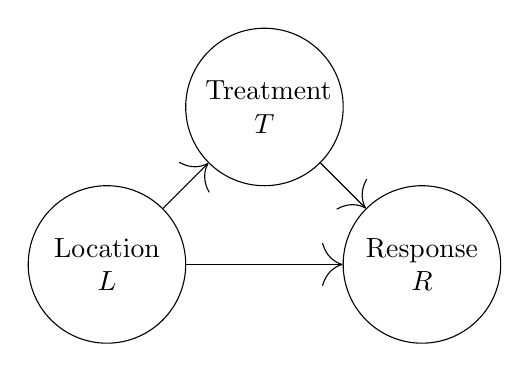
\begin{tikzpicture}[every node/.style={draw=black,shape=circle,minimum size=2cm,text width=1.5cm,align=center}]
    \node (type)[] at (0, 0) {Location \\ $L$};
    \node (treatment) at (2, 2) {Treatment \\ $T$};
    \node (recovery) at (4, 0) {Response \\ $R$};

    \path [-{>[scale=3.0]}] (type) edge (treatment);
    \path [-{>[scale=3.0]}] (type) edge (recovery);
    \path [-{>[scale=3.0]}] (treatment) edge (recovery); 
\end{tikzpicture}
\end{figure}

\begin{figure}
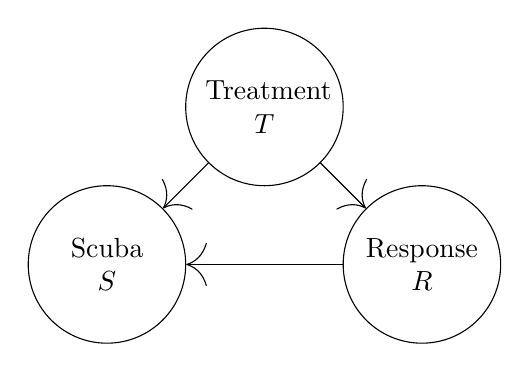
\begin{tikzpicture}[every node/.style={draw=black,shape=circle,minimum size=2cm,text width=1.5cm,align=center}]
    \node (lifestyle)[] at (0, 0) {Scuba \\ $S$};
    \node (treatment) at (2, 2) {Treatment \\ $T$};
    \node (recovery) at (4, 0) {Response\\ $R$};

    \path [-{>[scale=3.0]}] (recovery) edge (lifestyle);
    \path [-{>[scale=3.0]}] (treatment) edge (recovery); 
    \path [-{>[scale=3.0]}] (treatment) edge (lifestyle);
\end{tikzpicture}
\end{figure}

\begin{figure}
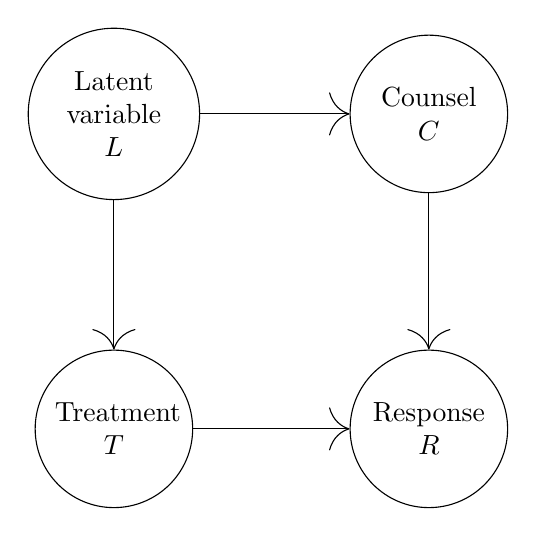
\begin{tikzpicture}[every node/.style={draw=black,shape=circle,minimum size=2cm,text width=1.5cm,align=center}]
    \node (treatment)[] at (0, 0) {Treatment \\ $T$};
    \node (recovery) at (4, 0) {Response \\ $R$};
    \node (latent) at (0, 4) {Latent variable \\ $L$};
    \node (counsel) at (4, 4) {Counsel \\ $C$};

    \path [-{>[scale=3.0]}] (treatment) edge (recovery);
    \path [-{>[scale=3.0]}] (latent) edge (treatment);
    \path [-{>[scale=3.0]}] (latent) edge (counsel);
    \path [-{>[scale=3.0]}] (counsel) edge (recovery);
\end{tikzpicture}
\end{figure}

\end{document} 
